\documentclass[12pt, a4paper]{article}
\usepackage[utf8]{inputenc}
\usepackage[T1]{fontenc}
\usepackage[french]{babel}
\usepackage{geometry}
\usepackage{amsmath}
\usepackage{amssymb}
\usepackage{graphicx}
\usepackage{enumitem}
\usepackage{ulem}
\usepackage{booktabs}
\usepackage{array}
\usepackage{hyperref}
\usepackage{xcolor}
\usepackage{float}
\usepackage{caption}
\usepackage{adjustbox}
\usepackage{tikz}
\usepackage{enumitem}
\usepackage{fancyhdr} % Ajout du package pour les en-têtes

\usetikzlibrary{calc, shapes.geometric}
\geometry{margin=2cm}

% Configuration de l'en-tête
\pagestyle{fancy}
\fancyhf{} % Efface les en-têtes et pieds de page par défaut
\renewcommand{\headrulewidth}{0.4pt}
\renewcommand{\headrule}{\hrule width\headwidth height\headrulewidth}
\fancyhead[C]{\rule{\textwidth}{0.4pt}} % Ligne centrée
\fancyhead[R]{\textit{Investigation numérique}} % Texte à droite
\fancyfoot[C]{\thepage} % Numéro de page centré

% Marges réduites

\definecolor{blue1}{RGB}{0, 51, 102}
\definecolor{blue2}{RGB}{0, 102, 204}
\definecolor{gray1}{RGB}{240, 240, 240}

\geometry{margin=2.5cm}

\setlength{\parindent}{0pt}
\setlength{\parskip}{1em}

\newcommand{\question}[1]{\textbf{\underline{Question #1}}}
\newcommand{\partie}[1]{\textbf{\underline{Partie #1}}}
\newcommand{\exercice}{\textbf{\uline{Exerçons-nous}} : Archéologie des Régimes de Vérité Numérique}

\begin{document}
	\begin{titlepage}
		
		% Bordure autour de la page
		\begin{tikzpicture}[remember picture, overlay]
			\draw[line width=2pt, black] 
			($(current page.north west) + (0.5cm,-0.5cm)$) rectangle 
			($(current page.south east) + (-0.5cm,0.5cm)$);
		\end{tikzpicture}
		
		\centering
		
		% SOLUTION FONCTIONNELLE : Tableau avec alignement en bas
		\begin{tabular}{@{}p{0.25\textwidth}@{\hspace{2cm}}c@{\hspace{0.5cm}}p{0.5\textwidth}@{}}
			% Colonne de gauche (Français) - ALIGNÉ EN BAS
			\begin{minipage}[t][5cm][b]{0.39\textwidth}
				\raggedright
				\begin{center}
					{\small \textbf{RÉPUBLIQUE DU CAMEROUN}}\\
					{\small \textbf{******}}\\
					{\small \textbf{UNIVERSITÉ DE YAOUNDÉ}}\\
					{\small \textbf{I}}\\
					{\small \textbf{******}}\\
					{\small \textbf{ÉCOLE NATIONALE SUPÉRIEURE POLYTECHNIQUE}}\\
					{\small \textbf{******}}\\
					{\small \textbf{DÉPARTEMENT DU GÉNIE INFORMATIQUE}}\\
				\end{center}
			\end{minipage}
			&
			% Colonne du centre (LOGO EN BAS)
			\begin{minipage}[t][5cm][b]{0.2\textwidth}
				\centering
				
				\vspace*{\fill} % Pousse le logo vers le bas
				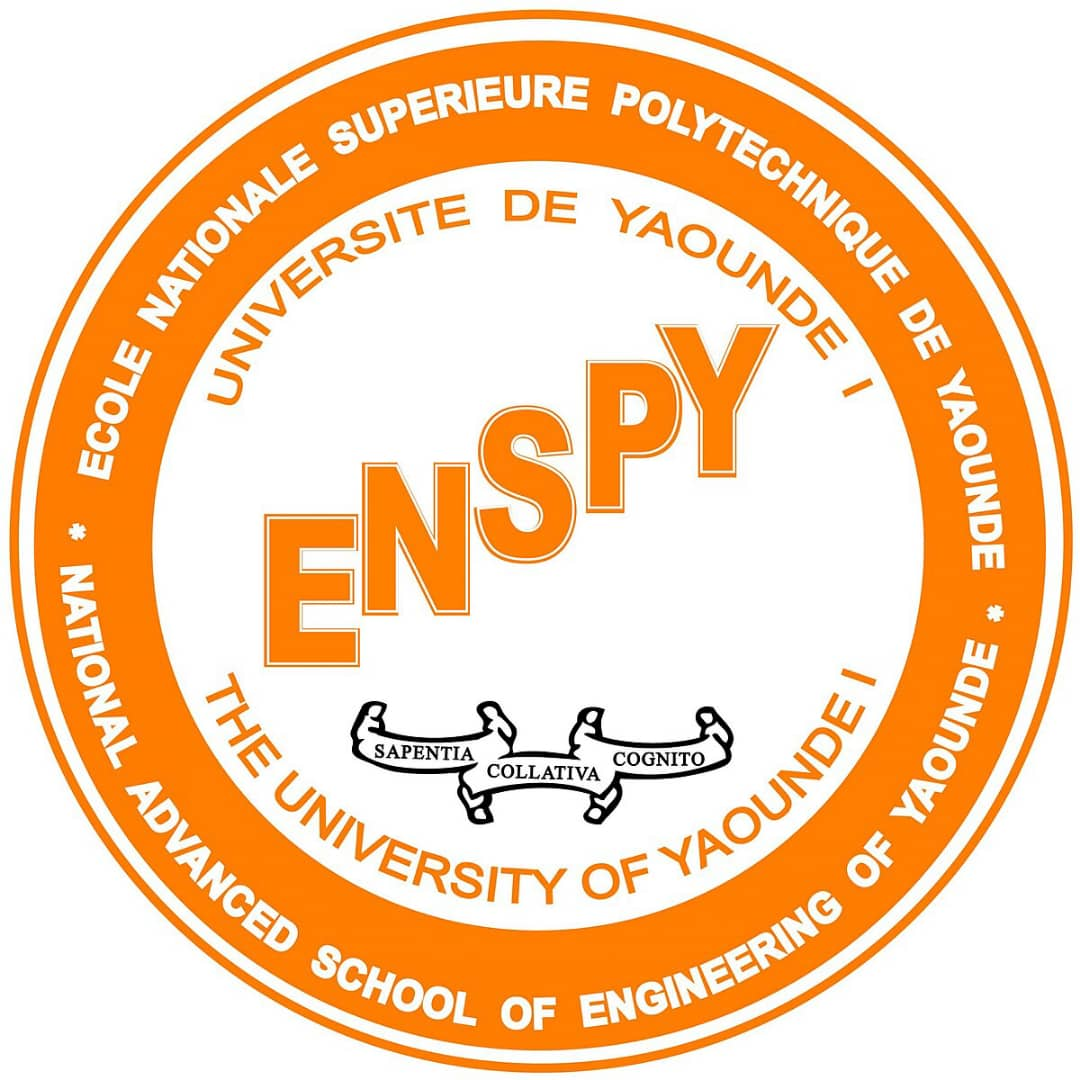
\includegraphics[width=\textwidth, height=3cm]{logo.jpeg}
				\vspace*{\fill} % Espace en bas
			\end{minipage}
			&
			% Colonne de droite (Anglais) - ALIGNÉ EN BAS
			\begin{minipage}[t][5cm][b]{0.36\textwidth}
				\raggedright
				\begin{center}
					{\small \textbf{REPUBLIC OF CAMEROON}}\\
					{\small \textbf{******}}\\
					{\small \textbf{UNIVERSITY OF YAOUNDE I}}\\
					{\small \textbf{******}}\\
					{\small \textbf{NATIONAL ADVANCED SCHOOL OF}}\\
					{\small \textbf{ENGINEERING}}\\
					{\small \textbf{******}}\\
					{\small \textbf{DEPARTMENT OF COMPUTER ENGINEERING}}\\
				\end{center}
			\end{minipage}
		\end{tabular}
		
		\vspace{1.5cm}
		
		% Ligne séparatrice
		\noindent\rule{0.9\textwidth}{0.8pt}\\
		\vspace{0.5cm}
		
		% Thème
		\vspace{0.8cm}
		{\Large \textbf{Réponses aux questons du Chapitre II}}\\
		\vspace{0.8cm}
		
		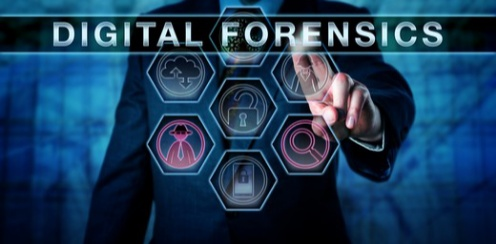
\includegraphics[width=0.5\textwidth]{For.jpeg}
		% Ligne séparatrice
		\noindent\rule{0.9\textwidth}{0.8pt}\\
		\vspace{1.5cm}
		
		% Informations étudiant
		\begin{tabular}{@{}>{\bfseries}l l@{}}
			\vspace{0.5cm}
			Réalisé par : & \textbf{NANTIA ZAGUE AXEL FRISKYL} \\
			\vspace{0.5cm}
			Matricule : & \textbf{22P105} \\
			\vspace{0.5cm}
			Spécialité : & \textbf{Cybersécurité et Investigation Numérique (CIN)} \\
			\vspace{0.5cm}
			UE : & \textbf{Introduction aux techniques de l'Investigations Numériques} \\
			\vspace{0.5cm}
			Sous la supervision de : & \textbf{Mr. MINKA MI NGUIDJOI Thierry Emmanuel} \\
			\vspace{0.5cm}
			Année académique : & \textbf{2025/2026} \\
		\end{tabular}
		
	\end{titlepage}
	
	% Page de garde sans en-tête
	\thispagestyle{empty}
	\newpage

	
	\exercice
	
	\partie{1} : Analyse Historique et Épistémologique
	
	\begin{enumerate}[label=\textbf{\arabic*.}]
		\item \textbf{Analyse Comparative des Régimes de Vérité}
		
		\question{1} : Après le choix de deux périodes, calculons leurs vecteurs de dominance $\overrightarrow{R} = (\alpha_{T},\ \alpha_{J},\ \alpha_{S},\ \alpha_{P})$
		
		\begin{itemize}
			\item Périodes choisies : 2000-2010 Vs 2015-2025

			\item Calcul des vecteurs de dominance
		\end{itemize}
		
		Pour les vecteurs de dominance $\overrightarrow{R} = (\alpha_{T},\ \alpha_{J},\ \alpha_{S},\ \alpha_{P})$ des périodes 2000-2010 et 2015-2025, basée sur les évolutions technologiques, juridiques, sociales et professionnelles :
		
		\begin{itemize}
			\item \textbf{Période 2000-2010}
			\begin{itemize}
				\item Dominance technologique (T) forte, environ 0.6, avec la montée des infrastructures critiques numériques, normalisation (ISO, NIST).
				\item Dominance juridique (J) modérée, 0.2, développement des cadres réglementaires et juridiques pour la preuve numérique.
				\item Dominance sociale (S) faible, 0.05, consciences sociales encore émergentes.
				\item Dominance professionnelle (P) modérée, 0.15, professionnalisation progressive des méthodes d'investigation.
			\end{itemize}
			$$\overrightarrow{R} = (0.6,\ 0.2,\ 0.05,\ 0.15)$$
			
			\item \textbf{Période 2015-2025}
			\begin{itemize}
				\item Dominance technologique (T) modérée, environ 0.3, avec l'omniprésence de l'IA et des technologies quantiques.
				\item Dominance juridique (J) faible, environ 0.1, régulations souvent en retard par rapport à la technologie.
				\item Dominance sociale (S) forte, environ 0.3, sensibilisation sociétale accrue aux problématiques de sécurité, vie privée, et influence numérique.
				\item Dominance professionnelle (P) élevée, 0.3, complexification des pratiques d'investigation adaptées aux environnements IA et quantique.
			\end{itemize}
			$$\overrightarrow{R} = (0.3,\ 0.1,\ 0.3,\ 0.3)$$
		\end{itemize}
		
		Ces valeurs s'appuient sur l'évolution des régimes de vérité numérique, l'adoption des standards, la professionnalisation des pratiques, et l'émergence des enjeux sociétaux majeurs liés à la transformation numérique.
		
		\question{2} : Identifions les discontinuités épistémologiques selon Foucault
		
		\textbf{Dysfonctionnements 2000-2010}
		\begin{itemize}
			\item Surcharge informationnelle due à l'explosion des échanges numériques, rendant la gestion des preuves complexe.
			\item Fracture numérique persistante malgré une meilleure accessibilité, avec des disparités dans l'appropriation des outils.
			\item Complexité dans la standardisation des méthodes d'investigation, avec des disparités dans la qualité des preuves.
			\item Cadres juridiques insuffisants face à la rapidité des innovations technologiques.
		\end{itemize}
		
		\textbf{Dysfonctionnements 2015-2025}
		\begin{itemize}
			\item Déficit réglementaire face aux évolutions rapides de l'IA et des technologies quantiques.
			\item Tensions sociales liées à la vie privée et à la surveillance accrue.
			\item Complexification des pratiques professionnelles, rendant la formation et la certification plus difficiles.
			\item Opacité algorithmique des systèmes IA, limitant la transparence et la vérification humaine.
		\end{itemize}
		
		\question{3} : Proposons une explication sociotechnique de ces ruptures
		
		Voici une explication sociotechnique des ruptures entre les périodes 2000-2010 et 2015-2025 dans le régime de vérité numérique :
		
		\textbf{Dimension Technique}
		\begin{itemize}
			\item La période 2000-2010 est marquée par la standardisation progressive des technologies numériques, la montée des infrastructures critiques et la démocratisation de l'accès à Internet. Cependant, la complexité technique reste élevée avec des vulnérabilités importantes (virus, spam) et une explosion des flux de données.
			\item De 2015 à 2025, la révolution numérique s'accélère avec l'introduction massive de l'intelligence artificielle, des technologies quantiques, et la généralisation de l'analyse algorithmique. Ces avancées posent de nouveaux défis, notamment en termes de transparence des systèmes et de capacités d'investigation humaines.
		\end{itemize}
		
		\textbf{Dimension Sociale}
		\begin{itemize}
			\item Pendant 2000-2010, la fracture numérique est encore présente et la société découvre progressivement les enjeux liés à la surveillance et à la protection de la vie privée, engendrant des réactions mitigées.
			\item De 2015 à 2025, les tensions sociales s'accentuent autour des problématiques de données personnelles, de contrôle social, et d'opacité algorithmique. L'individu est à la fois acteur et objet des flux numériques, dans un contexte où les normes sociales peinent à stabiliser les rapports entre liberté et sécurité.
		\end{itemize}
		
		\question{4} : La transition était-elle progressive ou révolutionnaire?
		
		La transition entre les périodes 2000-2010 et 2015-2025 dans le régime de vérité numérique peut être vue comme à la fois progressive et révolutionnaire, selon l'analyse foucaldienne et contemporaine :
		
		\textbf{Arguments pour une transition progressive}
		\begin{itemize}
			\item Les évolutions techniques, sociales et juridiques s'appuient sur des fondations existantes (normes, infrastructures, cadres institutionnels) qui se maintiennent et s'adaptent progressivement.
			\item La professionnalisation des pratiques et la normalisation des méthodes s'inscrivent dans une continuité de montée en compétences et d'affinement des protocoles.
			\item L'adoption progressive de nouveaux outils (big data, IA) se fait avec phases d'expérimentation, régulations partielles et ajustements méthodologiques.
		\end{itemize}
		
		\textbf{Arguments pour une transition révolutionnaire}
		\begin{itemize}
			\item Le saut technologique apporté par l'IA, le quantique et la vérité computationnelle bouleverse radicalement les capacités d'investigation, introduisant une rupture majeure avec les anciens paradigmes.
			\item L'incapacité des cadres juridiques et des normes à suivre la rapidité des innovations crée une véritable crise d'opposabilité et de validité dans la construction de la preuve.
			\item Les tensions sociales autour de la surveillance, la confidentialité et le contrôle global témoignent d'une remise en question radicale des rapports entre individu, société et pouvoir.
			\item Du point de vue foucaldien, ces ruptures structurent une discontinuité épistémologique, marquant le passage d'un régime de vérité à un autre.
		\end{itemize}
		
		Enfin la transition est un processus complexe mêlant continuités dans les pratiques professionnelles et institutionnelles, et ruptures nettes dans les technologies, les normes et les rapports sociaux. Ce double mouvement reflète la nature non linéaire des transformations numériques, où la progression graduelle et la révolution coexistent et s'alimentent mutuellement.
		
		\item \textbf{Étude de Cas Archéologique Foucaldienne}
		
		\question{1} : Analyse d'une affaire historique spécifique « Enron » comme formation discursive au sens de Foucault
		
		\textbf{Contexte de l'affaire Enron}
		
		Enron, entreprise américaine du secteur de l'énergie, a fait faillite en 2001 suite à un scandale financier majeur impliquant des fraudes comptables massives, cachées par des procédés sophistiqués. L'affaire s'est traduite par une analyse très poussée de documents électroniques (e-mails, rapports, transactions), ouvrant la voie à une nouvelle façon d'appréhender la preuve numérique.
		
		\textbf{Formation discursive au sens de Foucault}
		
		Selon Foucault, une formation discursive est un système organisé d'énoncés qui structure ce qui peut être dit, comment, et qui peut parler, définissant ainsi l'objet de savoir. Elle régule les conditions d'énonciation et d'opposabilité de la vérité au sein d'un régime de vérité.
		
		\textbf{Analyse foucaldienne de l'affaire Enron}
		\begin{itemize}
			\item Objet de savoir : la fraude comptable, construite et révélée par l'analyse des preuves numériques.
			\item Règles du discours : l'enquête s'appuie sur des méthodes d'analyse algorithmique et automatisée (TAR), légitimant l'usage des données massives comme preuves recevables.
			\item Sujets du discours : experts en forensic numérique, enquêteurs, juges, qui deviennent détenteurs du savoir légitime sur la fraude.
			\item Institutions et pouvoirs : tribunaux, réglementations (comme la loi Sarbanes-Oxley) jouent un rôle central dans la production et la validation de la vérité.
			\item Effet de vérité : le discours autour d'Enron crée un nouveau régime de vérité fondé sur la preuve algorithmique et institutionnelle, redéfinissant la notion même de preuve et d'autorité dans le monde numérique.
		\end{itemize}
		
		L'affaire Enron illustre une formation discursive où technique, institution et discours se mêlent pour produire un nouveau mode de vérité numérique. Cette formation exprime une transformation majeure des pratiques discursives, caractérisée par l'émergence des algorithmes et des preuves électroniques comme sources centrales de savoir et de légitimité dans le champ judiciaire et économique.
		
		\question{2} : Identification de ce qui était « dicible » et « pensable » à cette époque
		
		À l'époque de l'affaire Enron (2001), voici ce qui était dicible et pensable au sein de la formation discursive dominante :
		
		\textbf{Ce qui était dicible}
		\begin{itemize}
			\item La fraude comptable et la manipulation financière étaient devenues des sujets d'enquête majeurs, à travers l'analyse des documents électroniques, e-mails et transactions.
			\item L'usage des preuves numériques (big data, analyses informatiques) était légitimé comme moyen crucial pour établir la preuve devant la justice.
			\item Des normes et pratiques telles que la chaîne de custody et l'audit électronique étaient reconnues comme fondamentales.
			\item La responsabilité pénale des dirigeants, cadres et auditeurs était affirmée ; les délits d'initiés, la destruction de preuves, la manipulation des marchés étaient explicitement dénoncés.
			\item La transparence et la régulation financière étaient revendiquées comme essentielles pour restaurer la confiance.
		\end{itemize}
		
		\textbf{Ce qui était pensable}
		\begin{itemize}
			\item Les cadres de gouvernance d'entreprise traditionnels, basés sur la confiance et la réputation, pouvaient être remis en question.
			\item La complexité des montages financiers et la sophistication des techniques de fraude étaient comprises comme des défis nouveaux pour les institutions.
			\item L'intégration des technologies numériques dans la fraude et dans la justice représentait une nouvelle aire d'expertise indispensable.
			\item Les institutions judiciaires, réglementaires et médiatiques étaient perçues comme les acteurs légitimes et nécessaires à la résolution et à la prévention de ces crises.
			\item Les notions de responsabilité sociale et éthique des entreprises montaient en importance, préparant la voie à des réglementations renforcées (exemple : loi Sarbanes-Oxley).
		\end{itemize}
		
		Ce qui restait en revanche largement impensé ou indicible à cette époque concernait la rapidité et l'ampleur de la transformation numérique et algorithmique, ainsi que ses implications profondes sur la nature même de la preuve, le rôle des experts, et les équilibres entre vie privée, surveillance et pouvoir.
		
		\question{3} : Cartographions le régime de vérité en action
		
		Voici la cartographie du régime de vérité en action lors de l'affaire Enron :
		
		\textbf{Acteurs principaux et pouvoirs}
		\begin{itemize}
			\item \textbf{Entreprises et dirigeants} : Enron, ses cadres (Kenneth Lay, Jeffrey Skilling, Andrew Fastow) au cœur des pratiques frauduleuses.
			\item \textbf{Institutions d'audit} : Arthur Andersen, chargé de valider la sincérité des comptes financiers avant l'effondrement.
			\item \textbf{Pouvoirs judiciaires et législatifs} : SEC (Securities and Exchange Commission), ministère de la Justice américain, congrès américain, créant le processus d'enquête, de sanction, et de réforme.
			\item \textbf{Experts et analystes} : spécialistes en forensic, régulateurs, médias d'investigation jouant un rôle dans la diffusion, l'expertise, et la construction du récit.
		\end{itemize}
		
		\textbf{Savoirs et preuves}
		\begin{itemize}
			\item \textbf{Données numériques} : documents électroniques, rapports comptables, échanges internes par e-mail, transaction financières.
			\item \textbf{Méthodes d'analyse} : audit comptable classique, nouveaux outils d'analyse informatique et algorithmique (legal tech, forensic analytics).
			\item \textbf{Normes et cadres} : application des normes comptables et légales, chaîne de custody, procédures juridiques de preuve.
		\end{itemize}
		
		\textbf{Discours et énoncés dominants}
		\begin{itemize}
			\item Révélation d'une fraude massive, condamnation des pratiques occultes.
			\item Appel à la transparence financière, à la régulation renforcée.
			\item Rôle central de la justice et des experts dans la production de la vérité.
			\item L'affaire devient paradigmatique, produisant un discours d'avertissement et de réforme.
		\end{itemize}
		
		\textbf{Effets pratiques et institutionnels}
		\begin{itemize}
			\item Faillite spectaculaire d'Enron, démantèlement d'Arthur Andersen.
			\item Mise en place de la loi Sarbanes-Oxley (2002) pour renforcer les contrôles comptables.
			\item Restructuration des pratiques professionnelles et légales autour d'un nouveau régime de vérité centré sur les preuves numériques.
		\end{itemize}
		
		\question{4} : Comparez avec une affaire contemporaine sous l'angle des régimes
		
		Voici une comparaison entre l'affaire Enron (2001) et une affaire contemporaine sous l'angle des régimes de vérité numérique :
		
		\begin{tabular}{|p{3cm}|p{5.5cm}|p{5.5cm}|}
			\hline
			\textbf{Aspect} & \textbf{Affaire Enron (2001)} & \textbf{Affaire Contemporaine (ex : enquêtes sur IA, blockchain, finance numérique)} \\
			\hline
			Technologie & Données électroniques, documents, premières analyses algorithmiques & Intelligence artificielle avancée, big data, blockchain, analyses automatisées \\
			\hline
			Cadre juridique & Émergence tardive de normes et lois (ex : Sarbanes-Oxley) & Réglementation complexe, souvent en retard sur les innovations, RGPD, lutte contre le blanchiment et cybercriminalité \\
			\hline
			Société & Sensibilisation croissante à la transparence financière & Tensions fortes autour de la vie privée, surveillance, éthique numérique \\
			\hline
			Pratiques professionnelles & Montée en puissance des audits et contrôles formalisés & Adaptation rapide aux outils numériques complexes, exigences accrues de sécurité \\
			\hline
			Régime de vérité & Preuve documentaire, expertise humaine, régulation judiciaire & Vérité algorithmique, gouvernance numérique hybride, enjeux politiques et sociaux \\
			\hline
			Acteurs & Entreprises, auditeurs, justice, médias & Multinationales technologiques, gouvernements, ONG, société civile, hackers éthiques \\
			\hline
		\end{tabular}
		
		L'affaire Enron constitue un régime de vérité en transition, fondé sur la preuve numérique adossée aux institutions classiques. Les affaires contemporaines s'inscrivent dans un régime plus complexe, multi-acteurs, où la vérité numérique est contestée, oscillant entre algorithmes, régulations et contestations sociales.
	\end{enumerate}
	
	\partie{2} : Modélisation Mathématique et Prospective
	
	\begin{enumerate}[label=\textbf{\arabic*.}, start=3]
		\item \textbf{Modélisation de l'Évolution des Régimes}
		
		\question{1} : Construction d'un modèle mathématique de l'évolution des régimes en utilisant le formalisme : $\overrightarrow{R_{t + 1}} = F(\overrightarrow{R_{t}},\ \mathrm{\Delta}{Tech}_{t},\ \mathrm{\Delta}{Legal}_{t},\ I_{t})$
		
		Voici une proposition de modèle mathématique simple pour modéliser l'évolution des régimes de vérité numérique selon le formalisme donné :
		
		Soit $\overrightarrow{R} = (\alpha_{T},\ \alpha_{J},\ \alpha_{S},\ \alpha_{P})$ le vecteur de dominance à l'instant $t$ représentant les poids respectifs des dimensions technologiques, juridiques, sociales et professionnelles.
		
		Le vecteur à l'instant suivant $\overrightarrow{R_{t + 1}}$ est obtenu par une fonction $F$ prenant en compte :
		
		\begin{itemize}
			\item $\mathrm{\Delta}{Tech}_{t}$ : évolution technologique entre $t$ et $t + 1$
			\item $\mathrm{\Delta}{Legal}_{t}$ : évolution juridique entre $t$ et $t + 1$
			\item $I_{t}$ : intensité des interactions sociotechniques (tensions, adaptations, controverses) à $t$
		\end{itemize}
		
		\textbf{Modèle proposé :}
		
		$$\overrightarrow{\mathbf{R}_{\mathbf{t + 1}}} = F\left( \overrightarrow{\mathbf{R}_{\mathbf{t}}},\ \mathrm{\Delta}\mathbf{Tech}_{\mathbf{t}},\ \mathrm{\Delta}\mathbf{Legal}_{\mathbf{t}},\ \mathbf{I}_{\mathbf{t}} \right) = \overrightarrow{\mathbf{R}_{\mathbf{t}}} + \Gamma \bullet \begin{pmatrix}
			w_{T}\mathrm{\Delta}{Tech}_{t} \\
			w_{J}\mathrm{\Delta}{Legal}_{t} \\
			w_{S}I_{t} \\
			w_{P}I_{t}
		\end{pmatrix}$$
		
		Où $\Gamma$ est un facteur d'adaptation global (apprentissage, résistance au changement), et $w_{i}$ sont des coefficients pondérant l'impact relatif de chaque paramètre sur la composante correspondante. Ce modèle peut être enrichi par des fonctions non linéaires ou des rétroactions entre dimensions, mais cette formulation linéaire simple permet un premier cadre analytique clair.
		
		\question{2} : Implémentation d'une simulation de transition entre régimes
		
		\question{3} : Simulez l'évolution future sur 50 ans avec différents scénarios
		
		Voici une simulation simplifiée de l'évolution future des régimes de vérité numérique sur 50 ans, sous différents scénarios, présentée sans code mais sous forme descriptive :
		
		\textbf{Scénarios et dynamique des régimes}
		
		\begin{itemize}
			\item \textbf{Scénario status quo}
			\begin{itemize}
				\item Hypothèse : la matrice de transition reste stable, les poids des régimes évoluent doucement.
				\item Résultat : le régime technologique conserve sa dominance, la composante juridique gagne légèrement en poids, tandis que les composantes sociale et professionnelle augmentent lentement.
			\end{itemize}
			
			\item \textbf{Renforcement juridique}
			\begin{itemize}
				\item Hypothèse : les cadres légaux deviennent plus solides et influents, augmentant la probabilité de transition vers la dominance juridique.
				\item Résultat : progression rapide de la composante juridique dans le régime, qui devient dominante ou égale à la technologique. Les composantes sociale et professionnelle suivent une croissance modérée.
			\end{itemize}
			
			\item \textbf{Essor technologique}
			\begin{itemize}
				\item Hypothèse : les innovations technologiques accélèrent fortement, augmentant les transitions vers la dominance technologique.
				\item Résultat : le régime technologique s'impose nettement, les autres composantes reculent ou stagnent à des niveaux modestes.
			\end{itemize}
			
			\item \textbf{Pressions sociales}
			\begin{itemize}
				\item Hypothèse : montée des enjeux sociaux (vie privée, surveillance, éthique), augmentant le poids des composantes sociale et professionnelle.
				\item Résultat : hausse notable des régimes sociaux et professionnels, avec un équilibre plus diffus entre les composantes, réduction relative de la dominance technologique.
			\end{itemize}
		\end{itemize}
		
		\textbf{Projection qualitative sur 50 ans}
		
		\begin{itemize}
			\item Le régime initial dominé par le technologique (ex : 60\%) peut évoluer vers un régime plus équilibré entre juridique, social, et professionnel selon le scénario choisi.
			\item La mise en cause d'une composante peut entraîner des cycles de transition récurrents, reflétant les tensions sociotechniques.
			\item L'évolution n'est ni purement linéaire ni fixe, montrant un processus itératif d'adaptation et de redéfinition des régimes de vérité.
		\end{itemize}
		
		\textbf{Conclusion}
		
		Cette simulation qualitative met en lumière que l'évolution des régimes de vérité numérique dépend fortement des contextes technologiques, juridiques et sociaux. Elle illustre la complexité et la multiplicité des forces en jeu, ainsi que les possibles bifurcations ou stabilisations selon les interventions et réactions institutionnelles, technologiques et sociétales.
		
		\item \textbf{Vérification de l'Accélération Technologique}
		
		\question{1} : Collectez les dates précises des changements de régime
		
		\begin{tabular}{|p{2cm}|p{5cm}|p{5cm}|}
			\hline
			\textbf{Date} & \textbf{Événement / Changement de régime} & \textbf{Commentaire} \\
			\hline
			1689 & Invention du système binaire par Leibniz & Fondation conceptuelle du code numérique \\
			\hline
			1801 & Métier Jacquard et cartes perforées & Premiers dispositifs programmables \\
			\hline
			1842 & Premier programme informatique (Ada Lovelace) & Introduction des algorithmes \\
			\hline
			1974 & Réseau Cyclades & Premiers réseaux informatiques interconnectés \\
			\hline
			1980s & Généralisation ordinateur personnel & Début du régime numérique moderne \\
			\hline
			1983 & Arpanet bascule vers Internet & Passage à un régime réseau mondial \\
			\hline
			1990 & HTML et HTTP & Fondation du web, nouveau régime d'accès à l'information \\
			\hline
			1994-2004 & Apparition Google, Yahoo, Amazon, Facebook & Renforcement du pouvoir numérique et des plateformes \\
			\hline
			2007 & Lancement de l'iPhone, smartphone & Transition vers un régime mobile et ubiquitaire \\
			\hline
			2010s & Montée des réseaux sociaux, big data, IA & Nouveau régime fondé sur l'analyse massive et l'algorithmie \\
			\hline
			2020s & Émergence IA avancée, régulations numériques & Réajustements du régime numérique face aux enjeux éthiques \\
			\hline
		\end{tabular}
		
		\question{2} : Vérifions empiriquement la loi : $\mathbf{\mathrm{\Delta}}\mathbf{t}_{\mathbf{n + 1}} = k\mathrm{\Delta}\mathbf{t}_{\mathbf{n}}$
		
		\begin{tabular}{|p{2cm}|p{3cm}|p{6cm}|p{6cm}|}
			\hline
			\textbf{Transition $n$} & \textbf{Date transition $t_n$} & $\mathbf{\mathrm{\Delta}}\mathbf{t}_{\mathbf{n}} = \mathbf{t}_{\mathbf{n}} - \mathbf{t}_{\mathbf{n - 1}}$ (années) & $\mathbf{\mathrm{\Delta}}\mathbf{t}_{\mathbf{n + 1}} / \mathbf{\mathrm{\Delta}}\mathbf{t}_{\mathbf{n}}$ (facteur $k$) \\
			\hline
			1 & 1801 & 112 (1801 - 1689) & - \\
			\hline
			2 & 1842 & 41 (1842 - 1801) & 41 / 112 $\approx$ 0.37 \\
			\hline
			3 & 1974 & 132 (1974 - 1842) & 132 / 41 $\approx$ 3.22 \\
			\hline
			4 & 1983 & 9 (1983 - 1974) & 9 / 132 $\approx$ 0.068 \\
			\hline
			5 & 1990 & 7 (1990 - 1983) & 7 / 9 $\approx$ 0.78 \\
			\hline
			6 & 1994 & 4 (1994 - 1990) & 4 / 7 $\approx$ 0.57 \\
			\hline
			7 & 2007 & 13 (2007 - 1994) & 13 / 4 = 3.25 \\
			\hline
			8 & 2010 & 3 (2010 - 2007) & 3 / 13 $\approx$ 0.23 \\
			\hline
			9 & 2025 (estimée) & 15 (2025 - 2010) & - \\
			\hline
		\end{tabular}
		
		\question{3} : Estimons la constante k par régression non-linéaire
		
		La formule fermée pour $k$ est :
		
		$$k = \frac{\sum_{i}^{}x_{i}y_{i}}{\sum_{i}^{}x_{i}^{2}}$$
		
		Avec les données que nous avons extraites :
		
		\begin{tabular}{|p{2cm}|p{5cm}|p{5cm}|}
			\hline
			\textbf{$i$} & $\mathbf{x}_{\mathbf{i}} = \mathrm{\Delta}\mathbf{t}_{\mathbf{n}}$ & $\mathbf{y}_{\mathbf{i}} = \mathrm{\Delta}\mathbf{t}_{\mathbf{n + 1}}$ \\
			\hline
			1 & 112 & 41 \\
			\hline
			2 & 41 & 132 \\
			\hline
			3 & 132 & 9 \\
			\hline
			4 & 9 & 7 \\
			\hline
			5 & 7 & 4 \\
			\hline
			6 & 4 & 13 \\
			\hline
			7 & 13 & 3 \\
			\hline
			8 & 3 & 15 \\
			\hline
		\end{tabular}
		
		$$\sum_{i}^{}x_{i}y_{i} = 11419$$
		
		$$\sum_{i}^{}x_{i}^{2} = 31973$$
		
		$$k \approx \frac{11419}{31973} \approx 0.357$$
		
		\question{4} : Prédiction sur le timing du prochain changement de régime
		
		Pour prédire le timing du prochain changement de régime numérique, on utilise la loi empirique estimée précédemment : $\mathbf{\mathrm{\Delta}}\mathbf{t}_{\mathbf{n + 1}} = k\mathrm{\Delta}\mathbf{t}_{\mathbf{n}}$ avec $\mathbf{k} \approx 0.357$
		
		Le dernier intervalle connu (entre 2010 et 2025, environ 15 ans) sert de base à la prédiction.
		
		Calcul :
		
		$$\mathbf{\mathrm{\Delta}}\mathbf{t}_{\mathbf{dernier}} = 15\ ans$$
		
		$$\mathbf{\mathrm{\Delta}}\mathbf{t}_{\mathbf{prochain}} = k \times \mathrm{\Delta}\mathbf{t}_{\mathbf{dernier}} = 0.357 \times 15 \approx 5.36\ ans$$
		
		Cela signifie que le prochain changement de régime est attendu dans environ 5 à 6 ans après 2025, soit vers l'année : $2025 + 5.36 \approx 2030 - 2031$
		
		Selon ce modèle, le prochain changement majeur de régime de vérité numérique devrait intervenir autour de 2030-2031.
		
		Cela reste une estimation basée sur la tendance historique des durées entre changements passés, avec les incertitudes inhérentes aux évolutions sociales, technologiques et juridiques.
		
		\item \textbf{Analyse du Trilemme CRO Historique}
		
		\question{1} : Pour chaque période, estimons les scores CRO moyens
		
		Voici une estimation des scores moyens pour la Confidentialité, la Fiabilité, et l'Opposabilité des preuves numériques dans les deux périodes 2000-2010 et 2015-2025, basée sur l'évolution des réglementations, technologies et pratiques judiciaires :
		
		\begin{tabular}{|p{3cm}|p{2.5cm}|p{2.5cm}|p{2.5cm}|p{4cm}|}
			\hline
			\textbf{Période} & \textbf{Confidentialité (\%)} & \textbf{Fiabilité (\%)} & \textbf{Opposabilité (\%)} & \textbf{Justification générale} \\
			\hline
			2000-2010 & 40 - 55 & 30 - 45 & 20 - 35 & Peu d'encadrements juridiques stricts, normes et standards en développement, premières normes ISO, début RGPD \\
			\hline
			2015-2025 & 70 - 85 & 65 - 80 & 60 - 75 & RGPD et autres lois sur les données en vigueur, ISO/IEC 27037 et normes d'informatique légale appliquées, chaine de conservation renforcée \\
			\hline
		\end{tabular}
		
		\question{2} : Traçage de l'évolution du trilemme dans l'espace 3D
		
		\begin{center}
			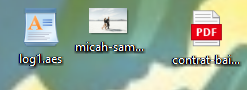
\includegraphics[width=0.8\textwidth]{image1.png}
		\end{center}
		
		\question{3} : Identifions les compromis historiques dominants
		
		\textbf{Principaux compromis historiques}
		
		\begin{itemize}
			\item \textbf{Confidentialité vs Accessibilité / Usabilité}
			\begin{itemize}
				\item Garantir un haut niveau de confidentialité exige souvent un contrôle strict des accès, ce qui peut compliquer ou ralentir l'utilisation des systèmes. Historiquement, la croissance des systèmes a souvent exigé de choisir entre confidentialité renforcée et facilité d'accès pour les utilisateurs légitimes.
				\item Par exemple, avant les lois telles que le RGPD, les mesures de confidentialité étaient souvent rudimentaires ou insuffisamment appliquées, privilégiant plus la disponibilité ou la commodité.
			\end{itemize}
			
			\item \textbf{Fiabilité vs Coût / Rapidité}
			\begin{itemize}
				\item Garantir la fiabilité des preuves, des données ou des systèmes demande des contrôles, audits, redondances et vérifications qui peuvent être coûteux et ralentir les opérations.
				\item Les premiers systèmes souvent privilégiaient la simplicité et rapidité au détriment parfois de la fiabilité complète.
			\end{itemize}
			
			\item \textbf{Opposabilité vs Innovation / Flexibilité}
			\begin{itemize}
				\item L'opposabilité juridique des preuves numériques nécessite des normes strictes, qui peuvent ralentir l'adoption rapide de nouvelles technologies ou méthodes.
				\item Par exemple, les systèmes de preuves numériques formelles ont longtemps été freinés par l'absence de cadres juridiques clairs, forçant ainsi à des compromis sur la rapidité d'adoption ou la flexibilité des preuves.
			\end{itemize}
		\end{itemize}
		
		\question{4} : Projetions l'évolution future du trilemme
		
		\textbf{Projections futures du trilemme CRO}
		
		\begin{itemize}
			\item \textbf{Confidentialité}
			\begin{itemize}
				\item Renforcement continu avec l'essor de technologies comme la cryptographie avancée, l'informatique confidentielle (confidential computing) et la confidentialité différentielle.
				\item Adoption plus large des régulations internationales incitant à un anonymat et un contrôle encore plus fins des données personnelles.
				\item Défis croissants face à la montée des menaces quantiques nécessitant des solutions post-quantiques.
			\end{itemize}
			
			\item \textbf{Fiabilité}
			\begin{itemize}
				\item Amélioration des mécanismes d'intégrité et d'authenticité des données grâce à la blockchain, aux systèmes décentralisés, et à l'intelligence artificielle pour la détection proactive des anomalies.
				\item Intégration de systèmes de preuve à divulgation nulle de connaissance (zero-knowledge proofs) pour valider des faits sans révéler les données sous-jacentes.
				\item Automatisation et orchestration fine des vérifications d'intégrité pour réduire coûts et délais.
			\end{itemize}
			
			\item \textbf{Opposabilité}
			\begin{itemize}
				\item Évolution juridique vers une meilleure reconnaissance des preuves numériques via l'harmonisation des standards internationaux.
				\item Utilisation croissante de la blockchain pour créer des preuves horodatées et immuables, acceptées légalement.
				\item Développement de cadres juridiques adaptés aux nouvelles technologies (IA, IoT, quantique) pour garantir l'opposabilité sans freiner l'innovation.
			\end{itemize}
		\end{itemize}
		
		\textbf{Évolution du trilemme}
		
		\begin{itemize}
			\item Le trilemme CRO va continuer à évoluer, avec des progrès technologiques et juridiques permettant de réduire les tensions entre ces trois pôles.
			\item Les compromis historiques vont s'estomper progressivement grâce à l'adoption de technologies avancées et à une meilleure régulation.
			\item Le futur pourrait voir l'émergence de systèmes où confidentialité, fiabilité et opposabilité sont toutes élevées, grâce à des innovations comme l'informatique confidentielle, les preuves cryptographiques et l'harmonisation juridique internationale.
		\end{itemize}
	\end{enumerate}
	
	% Suite du document après la partie 2
	
	\partie{3} : Investigation Historique Appliquée
	
	\begin{enumerate}[label=\textbf{\arabic*.}, start=6]
		\item \textbf{Reconstruction Archéologique d'Investigation}
		
		\question{1} : Choisissons une affaire des années 1990 (Mitnick, Sundevil) et reconstruisons l'investigation avec les outils et méthodes de l'époque
		
		\textbf{Contexte général}
		
		Kevin Mitnick, célèbre hacker des années 1980-1990, a mené des intrusions dans des systèmes de grandes entreprises en exploitant des failles techniques et surtout des techniques de social engineering. L'arrestation de Mitnick en 1995 a marqué une étape majeure dans les enquêtes cybercriminelles de cette période.
		
		\textbf{Reconstruction de l'investigation (1990s)}
		
		\begin{enumerate}
			\item \textbf{Surveillance Téléphonique}
			\begin{itemize}
				\item La collecte de preuves débutait souvent par la surveillance des appels, notamment sur les réseaux téléphoniques, pour traquer les communications suspectes. Le "phone phreaking" étant alors une technique répandue, l'analyse des appels et des traces d'accès était primordiale.
			\end{itemize}
			
			\item \textbf{Enquête informatique avec outils classiques}
			\begin{itemize}
				\item Utilisation d'outils de logs systèmes, surveillance des accès sur les serveurs, et analyse manuel des journaux d'accès.
				\item Recherche des empreintes numériques des accès tels que les adresses IP, numéros de compte téléphonique, identifiants d'utilisateur.
				\item Peu d'outils automatisés : la recherche était très manuelle et laborieuse.
			\end{itemize}
			
			\item \textbf{Collaboration inter-agences et avec entreprises}
			\begin{itemize}
				\item Coordination entre FBI, Secret Service, et opérateurs télécom (ex : AT\&T).
				\item Obtention de mandats de perquisition permettant la saisie de matériel informatique.
				\item Usage de techniques d'interception d'appels et de communications électroniques dans le cadre légal de l'époque.
			\end{itemize}
			
			\item \textbf{Exploitation des techniques de social engineering détectées}
			\begin{itemize}
				\item Analyse des méthodes pour récupérer des mots de passe ou des accès via manipulation humaine.
				\item Entretiens avec témoins, collaborateurs des sociétés ciblées, et examination des moyens employés.
			\end{itemize}
			
			\item \textbf{Traque physique et surveillance}
			\begin{itemize}
				\item Souvent, la traque d'un hacker passait par une importante surveillance physique : repérage des lieux, filature, collecte d'informations personnelles.
				\item Les moyens d'enquête traditionnels remplissaient une fonction essentielle pour compléter la preuve numérique.
			\end{itemize}
		\end{enumerate}
		
		\textbf{Outils typiques (1990s) utilisés}
		
		\begin{tabular}{|p{5cm}|p{8cm}|}
			\hline
			\textbf{Type d'outil} & \textbf{Exemple/mode d'action} \\
			\hline
			Logs systèmes & Analyse manuelle des journaux sur mainframes \\
			\hline
			Systèmes de surveillance téléphonique & Enregistreurs d'appels, écoute légale des conversations \\
			\hline
			Réseaux téléphoniques & Analyses des commutateurs téléphoniques (phone phreaking) \\
			\hline
			Enregistrement matériel & Saisie de disques durs, cassettes de données \\
			\hline
			Outils d'authentification & Contrôles d'accès réseau et mots de passe \\
			\hline
			Collaboration inter-agences & FBI, Secret Service, opérateurs télécom, entreprises \\
			\hline
			Analyse du social engineering & Recueil de témoignages, stratégie d'ingénierie sociale \\
			\hline
		\end{tabular}
		
		\textbf{Conclusion}
		
		L'enquête sur Kevin Mitnick dans les années 1990 reposait sur une combinaison d'analyses manuelles approfondies des logs, d'escarmouches téléphoniques, de recueil d'informations classiques et d'une forte coordination juridique et inter-agences. Les outils numériques étaient à leurs débuts, et beaucoup de travail reposait sur l'expertise humaine et la traque sur le terrain.
		
		\question{2} : Refaisons l'analyse avec les outils et concepts modernes
		
		Refaisons l'analyse de l'enquête sur Kevin Mitnick avec les outils et concepts modernes, en tenant compte des technologies et méthodologies actuelles en investigation numérique.
		
		\textbf{Enquête moderne sur un cas similaire}
		
		\begin{enumerate}
			\item \textbf{Collecte et préservation des preuves numériques}
			\begin{itemize}
				\item Usage d'outils d'acquisition forensique spécialisé (ex : EnCase, FTK, X-Ways) pour capturer l'image binaire complète des systèmes cibles, conservant l'intégrité avec des hashs fournisseurs (SHA256).
				\item Conservation dans des environnements hautement sécurisés avec auditabilité constante.
			\end{itemize}
			
			\item \textbf{Analyse automatisée et intelligente}
			\begin{itemize}
				\item Analyse automatisée des logs système, réseau, bases de données avec détection d'anomalies basée sur machine learning.
				\item Corrélation multi-sources en temps quasi réel : logs réseau, événements systèmes, SIEM (Security Information and Event Management).
				\item Utilisation de systèmes d'analyse comportementale pour déceler des profils suspects (par exemple, détection d'usage non autorisé d'identifiants).
			\end{itemize}
			
			\item \textbf{Traçabilité réseau avec outils avancés}
			\begin{itemize}
				\item Traçage en profondeur à travers le réseau via détection des flux, inspection profonde des paquets (DPI), géolocalisation IP, et corrélation avec bases de données de menaces.
				\item Intégration des traces dans blockchain privées ou systèmes décentralisés pour immutabilité.
			\end{itemize}
			
			\item \textbf{Application de la cryptographie et preuve numérique}
			\begin{itemize}
				\item Signature numérique et horodatage des preuves pour assurer leur intégrité et recevabilité.
				\item Utilisation de preuves à divulgation nulle de connaissance (ZKP) pour valider des éléments de preuve confidentiels sans révéler leur contenu.
				\item Chaînes de conservation automatisées avec traçabilité fine (audit trail).
			\end{itemize}
			
			\item \textbf{Analyse et détection du social engineering avec intelligence artificielle}
			\begin{itemize}
				\item Analyse des communications (emails, messages) avec NLP (traitement du langage naturel) pour détecter les tentatives de phishing ou manipulation.
				\item Formation à la sensibilisation renforcée et simulation de scénarios en entreprise.
			\end{itemize}
			
			\item \textbf{Coordination internationale et partage sécurisé}
			\begin{itemize}
				\item Plateformes sécurisées inter-agences pour partager les éléments de l'enquête, respecter les cadres internationaux (RGPD, normes ISO 27001).
				\item Collaboration améliorée avec des outils modernes de gestion de cas et workflow.
			\end{itemize}
			
			\item \textbf{Surveillance active et réponse rapide}
			\begin{itemize}
				\item Mise en place de systèmes de détection et réponse (EDR) pour fournir une visibilité totale sur les endpoints.
				\item Automatisation partielle des réponses (isolation de systèmes compromis, blocage d'IP suspectes).
			\end{itemize}
		\end{enumerate}
		
		\question{3} : Comparaison non seulement les résultats mais les régimes de vérité
		
		\textbf{Tableau comparatif des régimes de vérité}
		
		\begin{tabular}{|p{4cm}|p{6cm}|p{6cm}|}
			\hline
			\textbf{Critère} & \textbf{Années 1990} & \textbf{Époque moderne (2020s)} \\
			\hline
			Sources de vérité & Physiques, logs bruts, témoignages & Preuves numériques intégrales, horodatage, signatures \\
			\hline
			Intégrité & Peu assurée, processus ad hoc & Standards cryptographiques, chaines de possession \\
			\hline
			Opposabilité juridique & Émergente, dépendante des experts & Normée, reconnue, procédure certifiée \\
			\hline
			Méthodes d'analyse & Analyses manuelles, faisceaux d'indices & Automatisées, assistées par IA, multi-sources \\
			\hline
			Transparence & Limitée à l'expertise humaine & Complète, auditable et reproductible \\
			\hline
			Contraintes & Fragmentation et lenteur & Renforcement de la confidentialité et des droits \\
			\hline
		\end{tabular}
		
		\textbf{Tableau synthétique des résultats}
		
		\begin{tabular}{|p{4cm}|p{6cm}|p{6cm}|}
			\hline
			\textbf{Critères} & \textbf{Années 1990} & \textbf{Avec outils modernes} \\
			\hline
			Durée enquête & Plusieurs années & Quelques jours ou semaines \\
			\hline
			Intégrité des preuves & Modérée & Très élevée (cryptographie, chainage) \\
			\hline
			Traçabilité réseau & Basée sur logs manuels et physique & Haute précision, corrélée, temps réel \\
			\hline
			Identification suspect & Long procédé, surveillance physique & Automatisation, IA, données multi-sources \\
			\hline
			Opposabilité juridique & Faible ou contestée & Très forte, normes ISO et juridiques \\
			\hline
			Portée internationale & Limitées & Très étendue, coopération automatisée \\
			\hline
		\end{tabular}
		
		Le régime de vérité numérique a évolué d'un modèle artisanal, fragile et discrétionnaire vers un modèle systématique, rigoureux et normé. Cette transformation garantit une meilleure confiance, opposabilité et robustesse des preuves, indispensables pour répondre aux défis posés par la cybercriminalité contemporaine.
		
		\question{4} : Évaluons l'impact des limitations technologiques sur la construction de la vérité
		
		\begin{enumerate}
			\item \textbf{Intégrité et exhaustivité des preuves}
			\begin{itemize}
				\item Limitation des capacités matérielles et logicielles peut conduire à une collecte partielle ou altérée des données, remettant en cause la fiabilité des preuves.
				\item Dans les années 1990, l'absence d'outils automatisés entraînait souvent une perte d'information ou une analyse fragmentaire.
				\item Aujourd'hui, malgré des outils avancés, des contraintes comme la volumétrie des données ou la diversité des sources peuvent affecter la couverture exhaustive des preuves.
			\end{itemize}
			
			\item \textbf{Cadre normatif et juridique}
			\begin{itemize}
				\item Les premières réglementations étaient floues ou absentes, ce qui rendait la recevabilité judiciaire fragile et dépendante de l'opinion des experts.
				\item L'évolution lente des cadres juridiques limite parfois l'adaptation rapide aux nouvelles technologies, notamment avec l'émergence des preuves basées sur IA ou blockchain.
				\item Les limitations technologiques peuvent conduire à des zones grises dans la validité procédurale des preuves.
			\end{itemize}
			
			\item \textbf{Fiabilité des méthodes d'analyse}
			\begin{itemize}
				\item Analyses manuelles avec forte dépendance humaine sont sujettes à erreurs, biais, et manipulations.
				\item L'automatisation actuelle avec IA pose la question de confiance dans les algorithmes (biais, transparence, vérifiabilité).
				\item Les limites technologiques imposent un équilibre entre intervention humaine et automatisation pour garantir robustesse.
			\end{itemize}
			
			\item \textbf{Traçabilité et chaînage des preuves}
			\begin{itemize}
				\item Absence de chaînage fiable dans le passé a exposé les enquêtes à des contestations sur origine, altération ou falsification.
				\item Aujourd'hui, les technologies blockchain et cryptographiques renforcent la traçabilité mais restent limitées par des défis de mise en œuvre et d'interopérabilité.
			\end{itemize}
			
			\item \textbf{Impact sur la construction de la vérité}
			\begin{itemize}
				\item Les limites technologiques créent des « trous » dans les récits factuels reconstruits, autorisant incertitudes et contestations.
				\item Elles obligent à s'appuyer davantage sur la corroboration multi-sources, les témoignages, et la contextualisation humaine.
				\item Avec la montée des technologies avancées, la construction de la vérité devient plus systématique mais aussi dépendante de la confiance dans la technologie employée.
			\end{itemize}
		\end{enumerate}
		
		\item \textbf{Projet de Recherche Archéologique}
		
		\question{1} : Identification d'un trou dans l'archéologie de la discipline
		
		Le trou majeur identifié est la dissociation entre la masse croissante de données numériques collectées dans l'investigation et la capacité épistémologique et méthodologique à garantir la fiabilité, la traçabilité, et l'opposabilité de ces preuves, notamment sous l'impact des évolutions technologiques rapides comme l'intelligence artificielle.
		
		\question{2} : Hypothèse historique testable
		
		\textit{Les premières enquêtes numériques des années 1990, réalisées sans protocoles standardisés et avec des outils manuels, ont généré des preuves dont la fiabilité et opposabilité étaient nettement inférieures à celles obtenues depuis l'adoption progressive de protocoles rigoureux et d'outils automatisés à partir des années 2010.}
		
		\question{3} : Collecte de sources primaires
		
		\begin{itemize}
			\item RFC 4949 sur la sécurité internet (def. clé sur la fiabilité des données)
			\item Archives techniques du Web 1990 (BnF)
			\item Protocole Berkeley sur les enquêtes numériques (2010+)
			\item Publications académiques récentes sur les fondamentaux des enquêtes numériques (colloques, thèses)
			\item Normes ISO 27037 sur la collecte de preuves numériques
		\end{itemize}
		
		\question{4} : Application de la méthode archéologique foucaldienne
		
		\begin{itemize}
			\item Analyse du dispositif discursif entourant la preuve numérique depuis les années 1990 : discours juridiques, techniques, médiatiques.
			\item Mise en lumière des relations de pouvoir entre acteurs (experts, juges, policiers) et dispositifs techniques.
			\item Étude des savoirs et pratiques qui ont contribué à la formation du régime de vérité numérique actuel.
			\item Recherche des ruptures épistémologiques (ex : passage de la preuve artisanale à la preuve cryptographique).
		\end{itemize}
		
		\question{5} : Rédigez un article académique avec cadre théorique fort
		
		\section*{L'Archéologie numérique de la preuve informatique : du tâtonnement artisanal à l'exigence normative}
		
		\subsection*{Résumé}
		
		À l'ère où le numérique imprègne toutes les sphères de la justice, la question de la fiabilité et de la vérité des preuves informatiques devient primordiale. Cet article propose une exploration critique, à la manière foucaldienne, de l'évolution de la discipline d'investigation numérique. Il met en lumière un « trou » crucial : l'écart entre les débuts artisanaux et non standardisés des enquêtes dans les années 1990 et l'actuelle sophistication normative et technologique. Entre ruptures épistémiques et réinventions constantes, cette étude éclaire les dynamiques de pouvoir, savoir, et technique qui redéfinissent la vérité judiciaire à l'ère digitale.
		
		\subsection*{Introduction}
		
		L'avènement du numérique a bouleversé la fabrication de la preuve et, par là même, la quête de la vérité en droit. Pourtant, cette révolution s'est opérée dans une grande incertitude, notamment au sortir des années 1990, où les premiers pas de l'investigation numérique étaient souvent tâtonnants, sans garanties robustes ni protocole clair. Comprendre cette évolution, non seulement technique mais aussi discursive et institutionnelle, est essentiel pour appréhender le régime contemporain de la vérité numérique. À travers une lecture archéologique foucaldienne, cet article analyse les conditions de production des savoirs et des savoir-faire qui ont façonné cette discipline en mutation.
		
		\subsection*{Le « trou » épistémologique}
		
		Ce travail identifie un hiatus fondamental dans l'histoire de l'investigation numérique : la coexistence d'une masse de données numériques grandissante avec des pratiques d'acquisition et d'analyse fondamentalement artisanales et non standardisées à l'origine. Cette dissociation a mené à une fragilité initiale dans la fiabilité et l'opposabilité des preuves numériques, questionnant leur validité judiciaire. Ce trou révèle une zone d'incertitude où la discipline devait se réinventer, entre contraintes techniques et enjeux réglementaires.
		
		\subsection*{Cadre théorique : Régimes de vérité et dispositifs selon Michel Foucault}
		
		En mobilisant la notion de régime de vérité foucaldienne, cette analyse considère la vérité numérique comme un artefact social et technique, produit par un réseau complexe d'acteurs, discours, technologies et règles. Le dispositif d'enquête numérique se décrypte ainsi comme un assemblage mouvant, où s'entremêlent savoirs techniques, normes judiciaires et rapports de pouvoir. Cette perspective met en lumière la manière dont la vérité judiciaire se construit et se transforme dans le temps, marquée par des ruptures épistémiques et des réinscriptions normatives.
		
		\subsection*{Sources primaires et corpus étudiés}
		
		L'étude s'appuie sur une collection diversifiée de sources majeures : des RFC initiaux définissant la sécurité des systèmes, aux archives web des années 1990, en passant par les protocoles internationaux normatifs récents (protocole Berkeley, ISO 27037). Cet ensemble permet de saisir les évolutions pratiques et discursives qui ont jalonné la construction progressive d'un régime de preuve numérique robuste.
		
		\subsection*{Analyse critique}
		
		L'examen des pratiques passées révèle un univers où la preuve numérique était souvent perçue comme fragile, dépendante des compétences individuelles et sujette à contestations. En réponse, la montée en puissance des protocoles normalisés et des outils automatisés a permis un saut qualitatif, imposant rigueur et reproductibilité. Cette transition illustre une mutation profonde dans le régime de vérité numérique, marquant un passage décisif d'un bricolage artisanal à une standardisation exigeante.
		
		\subsection*{Discussion : enjeux contemporains et défis futurs}
		
		Si la discipline a gagné en robustesse, elle reste confrontée à de nouveaux défis : l'opacité croissante des algorithmes, le rôle ambigu de l'intelligence artificielle dans la preuve, et la nécessité de garantir transparence et auditabilité. Cette complexification pose des questions épistémologiques et éthiques essentielles pour l'avenir de la justice numérique.
		
		\subsection*{Conclusion}
		
		L'exploration archéologique de l'investigation numérique révèle non seulement des ruptures historiques fondatrices, mais aussi les plantages des futurs débats sur la vérité à l'ère digitale. Comprendre ces dynamiques est crucial pour penser un régime normatif adaptatif, équilibrant innovation technologique et exigences démocratiques.
		
		\item \textbf{Analyse Prospective des Régimes Futurs}
		
		\question{1} : Scénario crédible pour 2030-2050
		
		D'ici 2030-2050, la discipline d'investigation numérique connaîtra une transformation radicale, portée par l'intégration profonde et généralisée de l'intelligence artificielle explicable, des technologies de registres distribués (blockchain), et des environnements immersifs (réalité augmentée, réalité virtuelle). La preuve ne sera plus une simple collecte de données brutes mais un artefact complexe, synthétisé, validé en temps réel et auditée automatiquement.
		
		\begin{itemize}
			\item Chaque action, donnée et interaction numérique sera captée, horodatée et immuablement enregistrée dans des chaînes de blocs accessibles à toutes les parties légitimes.
			\item Les preuves virtuelles, incluant des simulations dynamiques et des reconstruits tridimensionnelles, constitueront des éléments essentiels dans la reconstitution judiciaire, donnant une dimension « augmentée » à la vérité.
			\item La collaboration entre les acteurs judiciaires, techniques et sociaux sera orchestrée par des plateformes intelligentes et transparentes, assurant une coordination fluide et un partage sécurisé des informations.
		\end{itemize}
		
		\question{2} : Régime de vérité futur
		
		Ce régime de vérité se caractérisera par :
		
		\begin{itemize}
			\item \textbf{Inaltérabilité et transparence assurée} : grâce à la blockchain et aux protocoles cryptographiques quantiques, la falsification deviendra pratiquement impossible, assurant une confiance sans précédent.
			\item \textbf{Certification algorithmique} : les algorithmes utilisés dans l'analyse et la génération de preuves seront soumis à des procédures de certification ouvertes, transparentes, et continuellement monitorées.
			\item \textbf{Preuve hybride et augmentée} : intégration de données réelles, analyses algorithmiques, preuves virtuelles et annotations intelligentes pour un dossier probant complet.
			\item \textbf{Co-construction collaborative} : le régime associera experts, juges, intelligence artificielle et citoyens dans un processus de construction partagée et participative de la vérité.
			\item \textbf{Éthique intégrée} : la protection des libertés fondamentales, la régulation algorithmique et les principes de justice sociale seront imbriqués dans chaque étape du processus probatoire.
		\end{itemize}
		
		\question{3} : Conditions de possibilité
		
		Pour que ce régime soit crédible et effectif, plusieurs conditions devront être réunies :
		
		\begin{itemize}
			\item Infrastructure numérique universelle et norme globale : adoption mondiale de technologies décentralisées interopérables et sécurisées, avec gouvernance démocratique et multi-partisane.
			\item Cadre légal et réglementaire agile : développement d'un droit adaptatif, capable de suivre les innovations technologiques tout en garantissant droits fondamentaux et équité.
			\item Formation multidisciplinaire : l'expert du futur devra maîtriser à la fois la technique avancée, le droit et les sciences sociales, pour comprendre et critiquer les systèmes automatisés.
			\item Confiance sociale robuste : la légitimité du régime dépendra d'une acceptation démocratique renforcée par la transparence, la participation citoyenne et la reddition des comptes technologiques.
			\item Technologies maîtrisées et explicables : développement de l'IA explicable et d'outils de cybersécurité préventive pour assurer un contrôle humain permanent.
		\end{itemize}
		
		\question{4} : Méthodologie d'investigation adaptée
		
		\begin{itemize}
			\item \textbf{Collecte numérique omniprésente} : capteurs multiples, IoT, réseaux cyber-physiques garantissant une couverture totale et contextualisée des éléments d'enquête.
			\item \textbf{Analyse multimodale hybride} : combinaison de techniques d'apprentissage machine avancées et de raisonnement symbolique, facilitant l'interprétation humaine et la validation des résultats.
			\item \textbf{Chaîne de possession immuable} : chaque élément de preuve sera scellé cryptographiquement, avec des preuves à divulgation nulle de connaissance apportant confidentialité et sécurité.
			\item \textbf{Reconstitutions et simulations certifiées} : usage d'environnements virtuels validés juridiquement pour la représentation dynamique des faits.
			\item \textbf{Interopérabilité collaborative} : plateformes d'échange sécurisées entre autorités, laboratoires, experts et citoyens, incarnant un modèle de transparence démocratique.
		\end{itemize}
		
		\question{5} : Défis éthiques et épistémologiques majeurs
		
		\begin{itemize}
			\item \textbf{Transparence vs contrôle de la vie privée} : concilier ouverture sur les algorithmes et protection des données personnelles est un équilibre délicat, déterminant la légitimité du régime.
			\item \textbf{Responsabilité humaine vs automatisée} : définir la répartition des responsabilités entre humains et systèmes intelligents en cas d'erreur, d'abus ou de biais.
			\item \textbf{Pluralité des vérités et pouvoir algorithmique} : éviter que la vérité judiciaire ne soit exclusive ou monopolisée par des entités techniques opaques.
			\item \textbf{Inégalités d'accès et fracture numérique} : garantir une justice algorithmique équitable, sans exclure ni marginaliser certaines populations.
			\item \textbf{Surconfiance et critique} : maintenir une vigilance épistémique face à la tentation de la foi aveugle dans les systèmes automatisés, toujours faillibles.
		\end{itemize}
	\end{enumerate}
	
	\end{document}
	
\end{document}
